% !TEX root = ../main.tex
\fancychapter{Solution}%
\label{chap:solution}
\cleardoublepage{}

\todo[inline]{{\bfseries TODO}: Vastly improve on this\ldots}

\noindent
Despite strides in enhancing performance and efficiency of geometric constraint
solving approaches, briefly discussed in \Cref{sec:intro.constraints}, the core
issue lies in the generality of geometric constraint solvers.  Although several
approaches employ efficient methods to find a solution, they resort to solving
potentially well-known problems generically when computationally lighter
solutions exist.  Instead of delegating the problem to a solver, a more
efficient approach would be to pinpoint the type of geometric constraint itself,
specializing a solution for several applicable entities.  Take the tangency
constraint as an example: positioning two circles tangent to each other or a
line tangent to an ellipse.  Depending on the inputs, these constraints might
have particularly efficient solutions for each case, in kind making the
computation more efficient.

Classical numerical methods constitute alluring alternatives to the predominant
graph-based approaches.  Having been studied for several decades, even if the
provided solution does not encompass all the possible values within the
problem's domain, they can be used to target specific problems efficiently.
Nonetheless, these suffer from robustness issues discussed in
\cref{sec:related.robustness}, effectively yielding inaccurate solutions if
precautions aren't taken.  A similar argument can be made about algebraic
methods.

This work aims to implement a series of geometric constraint primitives in an
already expressive \ac{TPL} to overcome the need for the specification of
unnecessary details when modeling geometrically constrained entities, promoting
an easier and more efficient usage.  Choosing to implement these in a \ac{TPL}
further avoids the poor scalability with increasing code complexity that arises
from what could be analogous specifications in a \ac{VPL}, a subject previously
discussed in \cref{sec:intro.ad}.

Moreover, by relying on an exact geometry computation library, one of the core
features of this solution lies in the capability of transparently dealing with
plenty of the previously addressed robustness issues.  The user can then resort
to these primitives, and, by composing them, elegantly specify the set of
geometric constraints necessary in order to produce the idealized model.  Since
the available primitives will implement specialized solutions for a finite set
of shapes the user can utilize in whichever combination possible during the
design process, the solution will be exempt of a generic solver component,
potentially boosting performance of design generation.

\Cref{fig:solution.arch} shows the typical \ac{AD} workflow and how the proposed
solution could be integrated with the \ac{AD} tool.  The encapsulated modules in
the figure represent the underlying computation library as an external
component, featuring the geometric constraint primitives library and the code
wrapping the computation library.

\begin{figure}[htbp]
  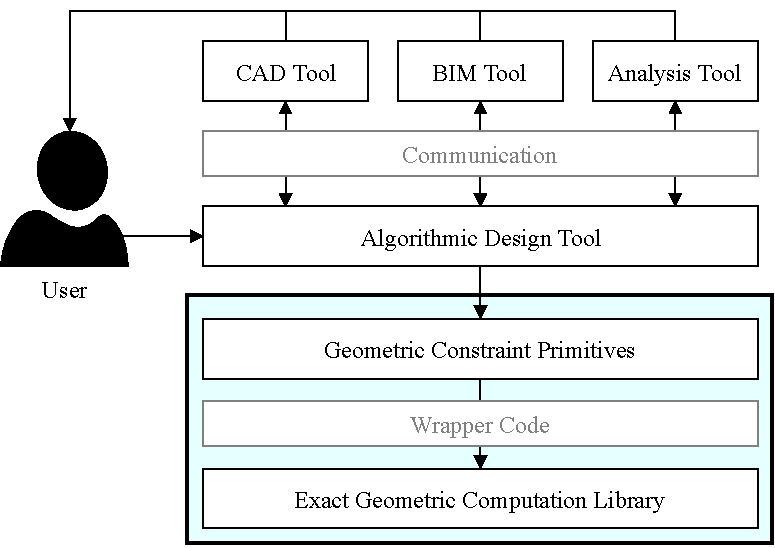
\includegraphics[width=\textwidth]{fig/solution-arch}
  \caption[Solution architecture within \acs{AD} workflow]{
    General overview of the solution's architecture encapsulated within the
    blue colored box beneath a depiction of the typical \ac{AD} workflow.}%
  \label{fig:solution.arch}
\end{figure}

\todo[]{Add foreword describing the following section(s)}
% !TEX root = ../../main.tex
\section{Implementation}%
\label{sec:solution.impl}

This section details implementation choices with regard to the chosen platforms
for realizing the initially proposed general solution architecture, previously
illustrated in \cref{fig:solution.arch}. Following a brief analysis, we expand
specifically on the concrete components corresponding to the ones within the
light blue rectangle.

Examining the \ac{AD} workflow portion of \cref{fig:solution.arch}, there are
depictions of \ac{CAD}, \ac{BIM}, and analysis tools, of which examples could be
Rhinoceros3D, Autodesk's Revit, and Radiance, respectively, with no particular
focus on any of them.  Digging a layer deeper, we find the \ac{AD} tool, which,
by means made available by the tools above it, produces models specific to those
tools from a description provided by the user.  The \ac{AD} tool we've chosen
was Khepri~\cite{Leitao:2019:GRUGEAV}, a text-based tool written in the Julia
programming language~\cite{Bezanson:2017:JAFANC}.  Khepri is the successor of
another text-based \ac{AD} tool named Rosetta~\cite{Leitao:2011:PGDCAD}, a tool
written in the Racket programming language~\cite{PLT:2010:Reference}.  It
follows that the \textit{Geometric Constraint Primitives} were implemented in
the Julia language as well, supported by an \textit{Exact Computation Geometry
Library}.  The library chosen for the effect was the
\acf{CGAL}~\cite{CGAL:2018}, a highly performant and robust geometric library
written in the C++ programming language~\cite{Stroustrup:2013:CPP}.

This language disparity between the \textit{Geometric Constraint Primitives}
module and the \textit{Exact Computation Geometry Library} requires a solution
for language interoperation.  In other words, we need to make \ac{CGAL}
available to the Julia language.  Fortunately, the Julia language already
possesses facilities that allow it to invoke functionality within libraries
written in the C~\cite{Kernighan:1988:C} or the
Fortran~\cite{Backus:1957:Fortran} programming languages.  This interfacing
mechanism is commonly known as \ac{FFI}.  It allows for the repurposing of
mature software libraries in foreign languages without the need for a complete
rewrite or adaptation.\footnote{The decision to include such a mechanism at the
language's core by the language designers makes it so the language can rapidly
evolve by avoiding reimplementing several facilities and software libraries in,
but not limited to, scientific and numerical computing areas.  Arguably, it may
be one of \textit{the} fundamental features that made the language as popular as
it is and kept it afloat, unlike other similar historical examples that might've
lacked such a mechanism.  \todo[inline]{Maybe expand on this with a concrete
example or so.  Could also be removed altogether}} This mechanism can also in
turn be leveraged and built upon to interface with other programming languages,
e.g., Java, Python, MATLAB, and, the one needed for our particular use-case,
C++.\footnote{There is an entire GitHub organization with projects dedicated to
foreign language interoperation at \url{https://github.com/JuliaInterop} (July
8, 2021)}

Overcoming the language interoperability hurdle, we can now start focusing on
the implementation of the \textit{Geometric Constraint Primitives}.  These
primitives build on top of the functionality available in \ac{CGAL}, some of
which is directly inherited from it, substantially helping us in the process,
e.g., intersections.  We further enriched the pool with a few more functions,
illustrating a constructive approach to \ac{GCS}, similar and inspired by the
approach of \textit{tkz-euclide} mentioned in
\cref{sec:related.constraints.tikz}.  By providing this abstraction over more
primitive functionality, we aimed to provide an easy to understand and utilize
set of tools so users can avoid reimplementing it themselves, which is an
error-prone process.  as levelling the playing field by working at a
conceptual level which is more familiar to and understood by traditional
\ac{CAD} software users rather than falling back to the more analytic approach
programming languages naturally offer.

The following sections will elaborate further on the components emphasized in
the previous paragraphs, adopting a bottom-up-like approach.  We'll discuss
\ac{CGAL} and what constructs and functionality it can provide to aid our goal,
as well as some added benefits of building on top of a very mature and
comprehensive library.  That will be followed by a section detailing how it was
possible to map said functionality to the Julia language, of which the result
was a Julia package aptly named \texttt{CGAL.jl}\footnote{Packages in the Julia
ecosystem are conventionally terminated with a \texttt{.jl} suffix, the
extension used for Julia files.  This is reminiscent of a familiar convention
followed in the Java ecosystem where libraries and tools are usually prefixed
with the letter \texttt{J}, e.g., \texttt{JUnit}, \texttt{JMeter},
\texttt{JDeveloper}, among others.}~\cite{Ventura:2019:CGAL.jl}.  Finally, we
showcase how we leveraged \texttt{CGAL.jl} to build the aforementioned
\textit{Geometric Constraint Primitives}, a set of functionality that implements
specialized yet comprehensible constructive approach solutions to \ac{GC}
problems.

\todo[inline]{Write said sections.}

% % !TeX root = ../../../main.tex
\subsection{Computational Geometry Algorithms Library}%
\label{sec:solution.impl.cgal}

\Ac{CGAL} is a software project that provides easy access to efficient and
reliable geometric algorithms in the form of a C++ library.  It is considered
the industry's \textit{de facto} standard geometric library, used in well-known
projects such as OpenSCAD\@.  It is also a very mature software library with
decades of Ph.D.-grade research results, still being actively maintained to this
day.  Being an open-source project, one can easily contribute to it by reporting
issues in the software as well as directly submitting patches.\footnote{The
library's source is hosted on GitHub at \url{https://github.com/CGAL/cgal}.  To
illustrate the ease with which one can contribute to the project, here is a pull
request the author submitted: \url{https://github.com/CGAL/cgal/pull/4705}.}

These factors, among others, justify our choice for our solution's
\geomlibrary{} component: we chose \ac{CGAL} because of its comprehensiveness
and decades of work invested in the production of a piece of highly mature
software, as well as the critical mass of maintainers behind it.  That is not to
say less mature software cannot be used in its stead, though it is unlikely it
can match \ac{CGAL}, be it in terms of performance, quality, or breadth.

\ac{CGAL} offers a multitude of data structures and algorithms, such as
triangulations, Voronoi diagrams, and convex hull algorithms, to name a few.
The library is broken up into three parts~\cite{CGAL:5.3:23LGK}:
\begin{enumerate}
  \item The kernel, which consists of geometric primitive objects and operations
  on these objects.  The objects are represented both as
  \begin{enumerate*}
    \item stand-alone classes parameterized by a representation class that
    specifies the underlying number types used for computation, and as
    \item members of the kernel classes, which allows for more flexibility and
    adaptability of the kernel;
  \end{enumerate*}
  \item Basic geometric data structures and algorithms, parameterized by traits
  classes that define the interface between the data structure or algorithm and
  the primitives they use;
  \item Non-geometric support facilities, such as circulators, random sources,
  and I/O support for debugging and for interfacing \ac{CGAL} with various
  visualization tools.
\end{enumerate}

Kernels in \ac{CGAL} are parametric, enabling the combination of kernels with
exact constructions or inexact constructions.  The latter are faster than the
former, but may produce inexact results due to \textit{roundoff} errors during
object construction.  In practice, however, inexact construction kernels suffice
for most of \ac{CGAL}'s algorithms.

\Cref{lst:solution.impl.cgal.pas} showcases an example of a very simple
\ac{CGAL} program, demonstrating the construction of points and a segment, and
performing some basic operations on them.

\begin{listing}[htbp]
  \caption[CGAL: Three points and one segment]{
    An example CGAL program illustrating how to construct some points and a line
    segment, and perform some basic operations on them.  It uses
    \mintinline{c}{double} precision floating point numbers for Cartesian
    coordinates.}\label{lst:solution.impl.cgal.pas}
  \inputminted{cpp}{cpp/points_and_segments.cpp}
\end{listing}

As mentioned, geometric primitive types are defined in the kernel.  The kernel
chosen in the example uses \texttt{double} precision floating point numbers for
the Cartesian coordinates of the point.

We can also see some predicates, such as testing the orientation of three
points, and constructions, like the distance\footnote{It is worth noting
\ac{CGAL} does \texttt{not} compute the absolute distance, offering instead to
compute the squared distance, as this avoids the additional square root
computation.  This preserves exactness and eliminates a potentially unnecessary
heavy computation.} and midpoint computation.  Predicates typically produce a
boolean logical value or one of a discrete set of possible results, whereas
constructions produce either a number or another geometric entity.

It is worth noting that floating point-based geometric computation can lead to
surprising results since we are relying on inexact constructions.  If one must
ensure that the numbers get interpreted at their full precision, all one has to
do is pick a kernel with exact constructions.  Revisiting
\cref{lst:solution.impl.cgal.pas}, it is as simple as switching the
\texttt{Simple\_cartesian} kernel with one the provides exact constructions,
e.g., \texttt{Exact\_predicates\_exact\_constructions\_kernel} or \texttt{Epeck}
for short.

Unfortunately, \ac{CGAL} is a terribly complex library under the hood,
presenting many challenges when it comes to mapping it to the Julia language.
Firstly, it is a C++ library.  Despite Julia's native capabilities for
interoperating with C, there's additional work to be done to reach C++ code.
Secondly, is problem of memory management, which differs between C/C++ and
Julia, potentially leading to memory leaks and other related issues if not
properly tended to.  Finally, \ac{CGAL} makes extensive use of C++ templates,
proving sometimes difficult to transparently map some of its constructs.

In the next section, we go over how we overcame these issues.

% % !TeX root = ../../../main.tex
\subsection{Computational Geometry Algorithms Library}%
\label{sec:solution.impl.cgal}

\Ac{CGAL} is a software project that provides easy access to efficient and
reliable geometric algorithms in the form of a C++ library.  It is considered
the industry's \textit{de facto} standard geometric library, used in well-known
projects such as OpenSCAD\@.  It is also a very mature software library with
decades of Ph.D.-grade research results, still being actively maintained to this
day.  Being an open-source project, one can easily contribute to it by reporting
issues in the software as well as directly submitting patches.\footnote{The
library's source is hosted on GitHub at \url{https://github.com/CGAL/cgal}.  To
illustrate the ease with which one can contribute to the project, here is a pull
request the author submitted: \url{https://github.com/CGAL/cgal/pull/4705}.}

These factors, among others, justify our choice for our solution's
\geomlibrary{} component: we chose \ac{CGAL} because of its comprehensiveness
and decades of work invested in the production of a piece of highly mature
software, as well as the critical mass of maintainers behind it.  That is not to
say less mature software cannot be used in its stead, though it is unlikely it
can match \ac{CGAL}, be it in terms of performance, quality, or breadth.

\ac{CGAL} offers a multitude of data structures and algorithms, such as
triangulations, Voronoi diagrams, and convex hull algorithms, to name a few.
The library is broken up into three parts~\cite{CGAL:5.3:23LGK}:
\begin{enumerate}
  \item The kernel, which consists of geometric primitive objects and operations
  on these objects.  The objects are represented both as
  \begin{enumerate*}
    \item stand-alone classes parameterized by a representation class that
    specifies the underlying number types used for computation, and as
    \item members of the kernel classes, which allows for more flexibility and
    adaptability of the kernel;
  \end{enumerate*}
  \item Basic geometric data structures and algorithms, parameterized by traits
  classes that define the interface between the data structure or algorithm and
  the primitives they use;
  \item Non-geometric support facilities, such as circulators, random sources,
  and I/O support for debugging and for interfacing \ac{CGAL} with various
  visualization tools.
\end{enumerate}

Kernels in \ac{CGAL} are parametric, enabling the combination of kernels with
exact constructions or inexact constructions.  The latter are faster than the
former, but may produce inexact results due to \textit{roundoff} errors during
object construction.  In practice, however, inexact construction kernels suffice
for most of \ac{CGAL}'s algorithms.

\Cref{lst:solution.impl.cgal.pas} showcases an example of a very simple
\ac{CGAL} program, demonstrating the construction of points and a segment, and
performing some basic operations on them.

\begin{listing}[htbp]
  \caption[CGAL: Three points and one segment]{
    An example CGAL program illustrating how to construct some points and a line
    segment, and perform some basic operations on them.  It uses
    \mintinline{c}{double} precision floating point numbers for Cartesian
    coordinates.}\label{lst:solution.impl.cgal.pas}
  \inputminted{cpp}{cpp/points_and_segments.cpp}
\end{listing}

As mentioned, geometric primitive types are defined in the kernel.  The kernel
chosen in the example uses \texttt{double} precision floating point numbers for
the Cartesian coordinates of the point.

We can also see some predicates, such as testing the orientation of three
points, and constructions, like the distance\footnote{It is worth noting
\ac{CGAL} does \texttt{not} compute the absolute distance, offering instead to
compute the squared distance, as this avoids the additional square root
computation.  This preserves exactness and eliminates a potentially unnecessary
heavy computation.} and midpoint computation.  Predicates typically produce a
boolean logical value or one of a discrete set of possible results, whereas
constructions produce either a number or another geometric entity.

It is worth noting that floating point-based geometric computation can lead to
surprising results since we are relying on inexact constructions.  If one must
ensure that the numbers get interpreted at their full precision, all one has to
do is pick a kernel with exact constructions.  Revisiting
\cref{lst:solution.impl.cgal.pas}, it is as simple as switching the
\texttt{Simple\_cartesian} kernel with one the provides exact constructions,
e.g., \texttt{Exact\_predicates\_exact\_constructions\_kernel} or \texttt{Epeck}
for short.

Unfortunately, \ac{CGAL} is a terribly complex library under the hood,
presenting many challenges when it comes to mapping it to the Julia language.
Firstly, it is a C++ library.  Despite Julia's native capabilities for
interoperating with C, there's additional work to be done to reach C++ code.
Secondly, is problem of memory management, which differs between C/C++ and
Julia, potentially leading to memory leaks and other related issues if not
properly tended to.  Finally, \ac{CGAL} makes extensive use of C++ templates,
proving sometimes difficult to transparently map some of its constructs.

In the next section, we go over how we overcame these issues.

% % !TeX root = ../../../main.tex
\subsection{Geometric Constraint Primitives}%
\label{sec:solution.impl.gcps}

Having overcome the language barrier between C++ and Julia, we can build our
\ac{GC} primitives on top of \texttt{CGAL.jl}.  Our implementation of the
\primitives{} is loosely inspired on tools like \texttt{tkz-euclide} and
Eukleides.  Both are based on Euclidean geometry, a constructive system where
the production of geometry can be done solely resorting to a straightedge and a
compass.  This makes programs described using these constructs easier to
understand and manually reproduce.

The following sections include a revisiting of our initially formulated example 
problems, described in \cref{sec:intro.examples}, and another set of primitives
that will be the driving force behind the case studies we go over later in
\cref{chap:eval}.

\subsubsection{Parallel lines}%
\label{sec:solution.impl.gcps.parallel}

Revisiting our earlier examples, we now showcase implementations for those
problems using our solution, accompanied by visualizations resorting to the
Khepri \ac{AD} tool.  \Cref{lst:solution.impl.gcps.parallel} shows a solution to
the ``parallel lines'' problem introduced in \cref{sec:intro.examples.parallel}.

\begin{listing}[htbp]
  \inputminted{julia}{jl/ex_parallel.jl}
  \caption[Parallel lines example using our solution]{
    Implementation of the parallel lines example illustrated in
    \cref{fig:intro.example.parallel} using Khepri alongside our solution.}%
  \label{lst:solution.impl.gcps.parallel}
\end{listing}

The sixth line in the program consists of the implementation of the primitive
construct.  The \texttt{parallel} function takes a line segment \texttt{l}, the
segment the resulting line is meant to be parallel to; and a point \texttt{p}
which the resulting line passes through.  We then build a new line segment whose
starting point is the given point \texttt{p}, and the end point is the result of
adding the difference between \texttt{l}'s endpoints to \texttt{p}, obtained
using \texttt{CGAL.jl}'s \texttt{to\_vector} function.

We then need to tell Khepri how to create objects our implementation can
understand by converting both the inputs and the resulting output.
\texttt{CGAL.jl} already contains a primitive shim of conversions between some
objects that facilitate this effort.\footnote{Ideally, the target \ac{AD} tool
would integrate our solution's constructs in a tighter more seamless fashion.}

Finally, we can use our primitive as seen in the listing's eighteenth line,
reproducing the same result. \Cref{fig:solution.impl.gcps.parallel} illustrates
the formulated program's output in AutoCAD, one of the visualization tools
Khepri supports.

\begin{figure}[htbp]
  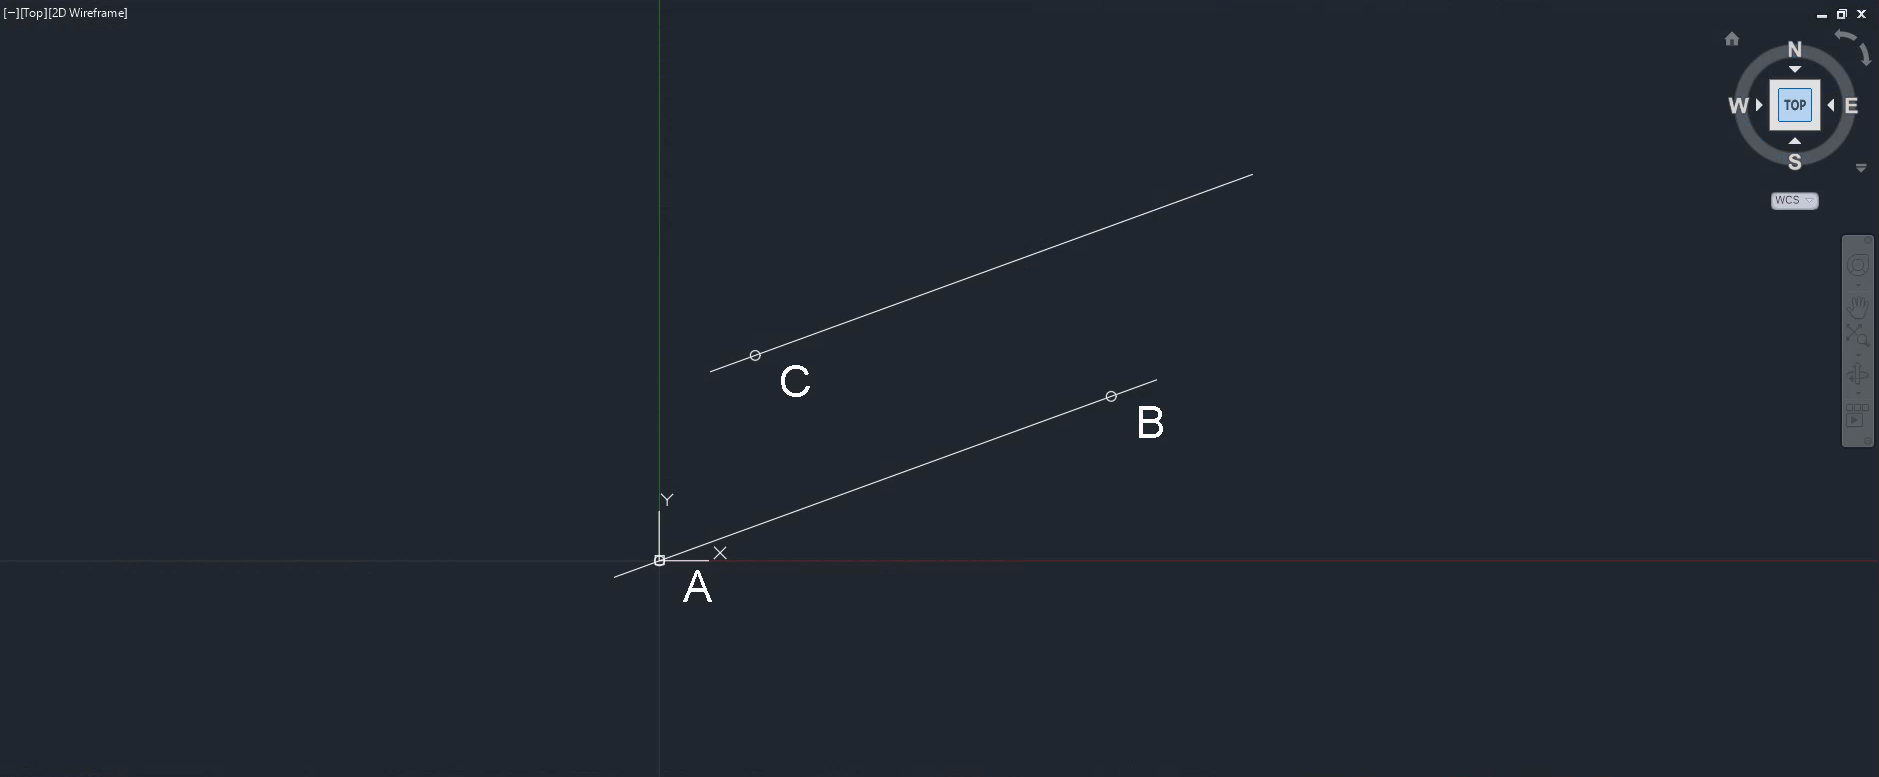
\includegraphics[width=\linewidth]{fig/autocad-parallel} 
  \caption[Parallel lines example using our solution]{
    Parallel lines example from \cref{sec:intro.examples.parallel} revisited
    using our solution's \texttt{parallel} primitive construct.  Output
    visualized in AutoCAD.}%
  \label{fig:solution.impl.gcps.parallel}
\end{figure}

\subsubsection{Circumcenter}%
\label{sec:solution.impl.gcps.circumcenter}

Regarding our circumcenter problem, introduced in
\cref{sec:intro.examples.circumcenter}, we initially solved it by intersecting
two of the three triangle sides' bisectors.  We can still approach the problem
that way, defining a \texttt{circumcenter} function similar to the one in
\cref{lst:solution.impl.gcps.circimpl}.

\begin{listing}[htbp]
  \begin{minted}[linenos=false]{julia}
  circumcenter(a, b, c) = intersection(bisector(a, b), bisector(b, c)) 
  \end{minted}
  \caption[Initial circumcenter solution]{
    Initial implementation of the \texttt{circumcenter} function.}%
  \label{lst:solution.impl.gcps.circimpl}
\end{listing}

However, this is one occasion where this functionality is already present in
\ac{CGAL}.  This is a simple yet perfect demonstration of one of our approach's
benefits with regard to repurposing a comprehensive library with plenty of
functionality, allowing us near-direct reuse without re-implementing it.

\Cref{lst:solution.impl.gcps.circumcenter} illustrates a solution to the
``circumcenter'' problem using \ac{CGAL}'s \texttt{circumcenter} function.  The
program's output can be seen in \cref{fig:solution.impl.gcps.circumcenter}.

\begin{listing}[htbp]
  \inputminted{julia}{jl/ex_circumcenter.jl}
  \caption[Circumcenter example using our solution]{
    Implementation of the circumcenter example illustrated in
    \cref{fig:intro.example.circumcenter} using Khepri alongside our solution.}%
  \label{lst:solution.impl.gcps.circumcenter}
\end{listing}

\begin{figure}[htbp]
  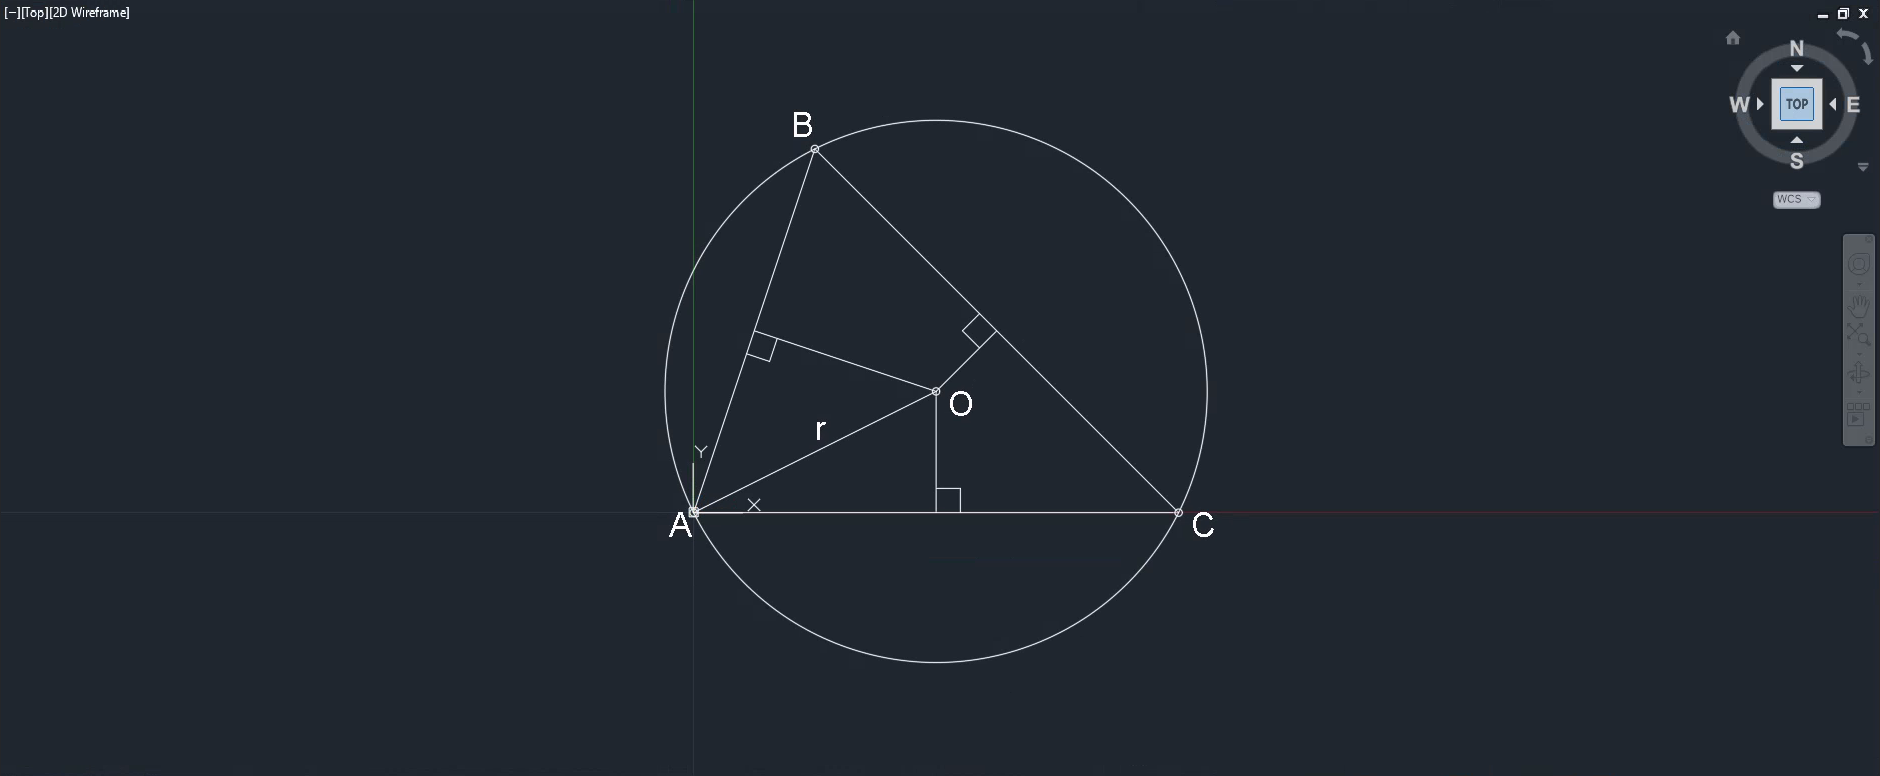
\includegraphics[width=\linewidth]{fig/autocad-circumcenter} 
  \caption[Circumcenter example using our solution]{
    Circumcenter example revisited using our solution's \texttt{circumcenter}
    primitive construct.  Output visualized in AutoCAD.}%
    \label{fig:solution.impl.gcps.circumcenter}
\end{figure}

\subsubsection{Circle tangent to a line}%
\label{sec:solution.impl.gcps.tangcirc2line}

Moving on to a set of problems that cannot as directly be solved by \ac{CGAL} is
that of tangencies.  Generally speaking, there are specific constructs available
in \ac{CGAL} that solve these problems.  However, we can once again repurpose
the ones we have and build on top of them.

This problem involves computing a circle that is tangent to an already existing
line.  Given the circle's center \texttt{o} and the line \texttt{l} we want the
circle to be tangent to, the tangent circle is such that its radius is the
minimal distance between its center point \texttt{o} and the line \texttt{l}.
The implementation of the problem's solution can be seen in
\cref{lst:solution.impl.gcps.tangcircle2line}.

\begin{listing}[htb]
  \begin{minted}[linenos=false]{julia}
  tangent_circle(o::Point2, l::Line2) = Circle2(o, squared_distance(o, l))
  \end{minted}
  \caption[Circle tangent to a line]{
    Implementation of the ``Circle tangent to a line'' problem.}%
  \label{lst:solution.impl.gcps.tangcircle2line}
\end{listing}

Notice this solution considers we are working with infinite lines, not
necessarily line \textit{segments} in general.  Were we to apply the same simple
approach to a line segment, the circle would end up tangent to the line segment
as well.  However, the resulting circle could be tangent to one of the segment's
endpoints instead of tangent to a point along the segment.  In some cases, the
latter behavior may be preferred, for which adjustments to the solution must be
made, such as indicating that there is no solution for the given center point.

We did not implement such a scenario regarding line segments, because much like
the other primitives, it was created to satisfy a specific use case's
requirements.  A potential solution to that specific problem could be obtained
reusing the \texttt{tangent\_circle} function, however.  We would then need to
verify if the circle would fall somewhere between the segment's endpoints.
Otherwise, there would not be a solution available.

\subsubsection{Tangent circles}%
\label{sec:solution.impl.gcps.tangentcircles}

Another instance of tangency is that of two circles tangent to each other.  This
proves to be a relatively more complex problem due to how the circles may be
positioned.

Given two circles \texttt{c\textsubscript{1}} and \texttt{c\textsubscript{2}},
and a vector \texttt{v} used to indicate the point of tangency on
\texttt{c\textsubscript{1}}, we draw a circle centered on said point with the
same radius as \texttt{c\textsubscript{2}} and intersect it with a ray
\texttt{r'} originating from the former circle's center, giving us a point
\texttt{f}.  This ray may be directed in one of two ways, determining if the
resulting circle contains both circles or not.  We then compute the bisector
\texttt{b} between \texttt{f} and \texttt{c\textsubscript{2}}.  We test if we
are in a situation where the resulting circle would instead turn out to be a
line.  If that is the case, we produce an error.  Otherwise, we construct the
tangent circle.

\Cref{lst:solution.impl.gcps.tangentcircles} contains the solution to the
problem, assisted by our own definition of the intersection function between a
circle and a ray, listed in \cref{lst:solution.impl.gcps.circrayint}.

\begin{listing}[htb]
  \inputminted[firstline=11]{julia}{jl/tangent_circles.jl}
  \caption[Tangent circles]{
    Implementation of the ``Tangent circles'' problem.}%
  \label{lst:solution.impl.gcps.tangentcircles}
\end{listing}

\begin{listing}
  \inputminted[lastline=9]{julia}{jl/tangent_circles.jl}
  \caption[Circle-Ray intersection]{
    Implementation of the intersection between a circle and a ray.}%
  \label{lst:solution.impl.gcps.circrayint}
\end{listing}

\subsubsection{Tangent lines between circles}%
\label{sec:solution.impl.gcps.tanglines2circles}

Another problem that surfaced in a case study earlier illustrated in
\cref{fig:intro.chair} is that of computing tangent lines between two circles.
It is a slightly more complex problem for which there is no obvious solution.
Fortunately, a constructive solution to this problem already
exists,\footnote{\url{https://en.wikipedia.org/wiki/Tangent_lines_to_circles\#Synthetic_geometry}}
an approach our implementation is based on.

This problem's complexity lead us to break it into two different problems.
First, we must determine the lines tangent to a circle that pass through a given
point (\cref{lst:solution.impl.gcps.tanglines2circles}).  Then, repurposing the
solution to that problem, we solve the overarching problem of determining the
lines tangent between circles (\cref{lst:solution.impl.gcps.tanglines2circle}).
This is another example of how we can compose a smaller set of primitives to
solve a larger problem.

\begin{listing}[htbp]
  \inputminted[firstline=2,lastline=16]{julia}{jl/circ_tangent_lines.jl}
  \caption[Tangent lines to a circle]{
    Implementation of the ``Tangent lines to a circle'' sub-problem.}%
  \label{lst:solution.impl.gcps.tanglines2circles}
\end{listing}

\begin{listing}[htbp]
  \caption[Tangent lines between circles]{
    Implementation of the ``Tangent lines between circles'' problem by way of
    composition with the solution of ``Tangent lines to a circle''.}%
  \label{lst:solution.impl.gcps.tanglines2circle}
  \inputminted[firstline=18,lastline=59]{julia}{jl/circ_tangent_lines.jl}
\end{listing}

Our implementation returns the results in a deterministic way, facilitating
result choice.  The line segments are oriented from \texttt{c\textsubscript{1}}
to \texttt{c\textsubscript{2}}, with the internal tangents surrounded by the
external tangents, sorted in a counterclockwise orientation.


